\documentclass{scrreprt}

\usepackage{aligned-overset}
\usepackage{amsmath}
\usepackage{amssymb}
\usepackage{bm}
\usepackage{chngcntr}
\usepackage[shortlabels]{enumitem}
\usepackage{hyperref}
\usepackage[utf8]{inputenc}
\usepackage{mathtools}
\usepackage{physics}
\usepackage{tabularx}
\usepackage{titling}
\usepackage{fancyhdr}
\usepackage{xfrac}
\usepackage[table]{xcolor}
\usepackage{pgfplots}

%% See https://tex.stackexchange.com/a/44954
\newcounter{myequation}
\makeatletter
\@addtoreset{equation}{myequation}
\makeatother

%% Fix equation numbering for scrreprt class.
\counterwithout{equation}{chapter}

\pgfplotsset{compat = newest}
\usepgfplotslibrary{patchplots}
\usetikzlibrary{intersections}
\usetikzlibrary{shapes}
\usetikzlibrary{shapes.geometric}
\usetikzlibrary{patterns}
\usepgfplotslibrary{fillbetween}

\author{Karsten Lehmann}
\date{SoSe 2021}
\title{Prüfungsvorbereitung Analysis - Weiterführende Konzepte}

\fancypagestyle{main}{
  \fancyhf{}
  \lhead{\thetitle}
  \rhead{\theauthor}
  \lfoot{\thedate}
  \rfoot{Seite \thepage}
}
\fancypagestyle{plain}{
  \fancyhf{}
  \lhead{\thetitle}
  \rhead{\theauthor}
  \lfoot{\thedate}
  \rfoot{Seite \thepage}
}
\pagestyle{main}

\newcommand\skalprod[1]{\left\langle #1 \right\rangle}
\newcommand\nnorm[1]{\left\lvert\left\lvert\left\lvert #1 \right\rvert\right\rvert\right\rvert}

% Hide the chapter and section numbers
\renewcommand\thechapter{}
\renewcommand\thesection{}

\begin{document}
\tableofcontents
\newpage
\chapter{Aufgaben}
\section{Blatt 03 - Aufgabe 4}

Sei $\lVert \cdot\, \rVert_p, 1 \leq p \leq \infty$ die $p$-Norm auf $\mathbb{R}^N$
\begin{enumerate}[a)]
\item Skizzieren Sie in $\mathbb{R}^2$ die Einheitskugeln für
  $p = 1, 2, \infty$, d.h., skizzieren Sie die Mengen
  \[
    B_p[0, 1] = \left\{ x \in \mathbb{R}^N \middle| \lVert x \rVert_p \leq 1 \right\}
    \text{ bzw. }
    B_p(0, 1) = \left\{ x \in \mathbb{R}^N \middle| \lVert x \rVert_p \leq 1 \right\}
  \]

  \item Beweisen Sie, dass für $1 \leq p \leq q \leq \infty$ und
    $x \in \mathbb{R}^N$ folgende Ungleichungen gelten:
    \[
      \colorbox{orange!50}{$\norm{x}_{\infty}$}
      \leq \colorbox{green!20}{$\norm{x}_q \leq \norm{x}_p$}
      \leq \colorbox{purple!50}{$N^{\sfrac{1}{p}} \norm{x}_{\infty}$}
    \]

  \item Zeigen Sie unter Verwendung der Hölder-Ungleichung, dass für
    $1 < p < q < \infty$ und $x \in \mathbb{R}^N$ die folgende Ungleichung
    gilt:
    \[
      \lVert x \rVert_p \leq N^{\frac{1}{p} - \frac{1}{q} \lVert x \rVert_q}
    \]
  \end{enumerate}

\section{Blatt 03 -  Aufgabe 5}

Sei $d_2 \colon \mathbb{R}^2 \times \mathbb{R}^2 \to \mathbb{R}$ die
euklidische Metrik. Für $x, y \in \mathbb{R}^2$ sei
\[
  d(x, y) \coloneqq \frac{d_2(x, y)}{1 + d_2(x, y)}
\].
\begin{enumerate}[a)]
\item Beweisen Sie, dass $\left( \mathbb{R}^2, d \right)$ ein metrischer
  Raum ist.
\item Sei $\lVert x \rVert \coloneqq d(x, 0)$.
  Ist dann $\left( \mathbb{R}^2, d \right)$ ein normierter Raum (Begründung)?
\item Geben Sie die Kugeln $B_d(0, 1)$ und $B_d\left( 0, \frac{1}{2} \right)$
  an. Sind diese Mengen \colorbox{purple!20}{konvex}?
\end{enumerate}

\section{Blatt 03 - Hausaufgabe 3}

Sei $M$ eine nichleere Menge.
\begin{enumerate}[a)]
\item Zeigen Sie, dass durch $d(x, y) \colon \begin{cases}
    1 & \text{für $x \ne y$} \\
    0 & \text{für $x = y$} \\
  \end{cases}$ eine Metrik auf $M \times M$ definiert ist.

\item Geben Sie für ein festes $x \in M$ und $r > 0$ die Kugeln
  $B(x, r) = \qty{ y \in M \middle| d(x, y) < r}$ und
  $B[x, r] = \qty{ y \in M \middle| d(x, y) \leq r}$ an.

\end{enumerate}

\textbf{Hinweis:} Die so definierte Metrik $d$ heißt diskrete Metrik von $M$.

\section{Blatt 04 - Aufgabe 3}

Wir betrachten den normierten Raum $(\mathbb{R}^2, \norm{\cdot}_2)$.
Skizzieren Sie die folgenden Mengen $A \subseteq \mathbb{R}^2$ und untersuchen Sie,
ob diese offen, abgeschlossen bzw. Umgebungen des Nullpunktes sind.
Geben Sie jeweils das Innere $\mathring A$, den Abschluss $\overline{A}$,
den Rand $\partial A$ und die isolierten Punkte dieser Mengen an.

\begin{enumerate}[(i)]
\item $A = B(x, r)$ mit $x \in \mathbb{R}^2$ und $r > 0$
\item $A = B[x, r] = \qty{y \in \mathbb{R}^2 \middle| \norm{x - y}_2 \leq r}$ mit $x \in \mathbb{R}^2$ und $r > 0$
\item $A = \qty{y \in \mathbb{R}^2 \middle| \norm{x - y}_2 > r}$ mit $x \in \mathbb{R}^2$ und $r > 0$
\item $A = \qty{x = \qty(x_1, x_2) \in \mathbb{R}^2 \middle| \qty(x_1 > -1) \land \qty(x_2 \geq -1)}$
\item $A = \qty{ x_n = \qty(\frac{1}{n}, 0) \middle| n \in \mathbb{N}}$
\end{enumerate}

\section{Blatt 04 - Aufgabe 4}

Wir betrachten den metrischen Raum $(\mathbb{R}, d)$ mit $d(x, y) = \abs{x - y}, x, y \in \mathbb{R}$.
Die Menge $M = [0, 1) \cup \qty{\frac{3}{2}} \cup(2, 3)$ sei mit der induzierten Metrik
$d_M \coloneqq d|_{M \times M}$ versehen, so dass der metrische Raum $\qty(M, d_M)$ entsteht.

\begin{enumerate}[a)]
\item Geben Sie die Mengen $B_d\qty(\frac{3}{2}, r)$ und $B_{d_M}\qty(\frac{3}{2}, r)$
  für $r = 1$ bzw. $r = \frac{1}{2}$ an.

\item Welche der folgenden Mengen $A_k$ sind offen/abgeschlossen in den Räumen $(\mathbb{R}, d)$
  bzw. $(M, d_M)$, wobei $A_1 = [0, 1)$, $A_2 = [0, 1) \cup \qty{\frac{3}{2}}$, $A_3 = (2, 3)$,
  $A_4 = M$ gilt?

\item Ist $\qty(M, d_M)$ ein vollständiger metrischer Raum?
\end{enumerate}

\section{Blatt 04 - Aufgabe 7}

Untersuchen Sie, ob die folgenden Folgen $\qty(x_n)$ aus $\mathbb{R}^2$
beschränkt bzw. konvergent bzgl. der Euklidischen Norm bzw. Metrik sind.
Ermitteln Sie gegebenenfalls den Grenzwert dieser Folgen.
\begin{enumerate}[a)]
\item $x_n = \qty(\frac{(-1)^n}{n}, \sin\qty(\pi + \frac{1}{n}))$
\item $x_n = \qty(\frac{1}{n}, n - \frac{1}{n})$
\item $x_n = \qty(\cos(\pi n), \frac{1}{n} \sin\qty(\frac{\pi}{2}n))$
\end{enumerate}

\section{Blatt 04 - Hausaufgabe 1}

Wir betrachten $D = \mathbb{Q}$ als Teilmenge von $\mathbb{R}$.
Zeigen Sie, dass $\mathring{\mathbb{Q}} = \emptyset$, $\overline{\mathbb{Q}} = \mathbb{R}$
und $\partial \mathbb{Q} = \mathbb{R}$ gelten.

\section{Blatt 04 - Hausaufgabe 3}

Sei $M \coloneqq (0, \infty)$ und $d \colon M \times M \to \mathbb{R}$ sei definiert durch
$d(x, y) = \abs{\ln x - \ln y}$.

\begin{enumerate}[(i)]
\item Beweisen Sie, dass $(M, d)$ ein metrischer Raum ist.
\item Sei $d|_M$ die von $(\mathbb{R}, \abs{\cdot})$ induzierte Metrik auf $M$.
  Untersuchen Sie, ob die Räume $(M, d)$ und $\qty(M, d|_M)$ vollständig sind. \\
\end{enumerate}

\section{Blatt 04 - Hausaufgabe 4}

Untersuchen Sie, ob die folgenden Folgen $\qty(x_n)$ aus $\mathbb{R}^3$ beschränkt bzw.
konvergent bezüglich der Euklidischen Norm sind.
Geben Sie gegebenfalls den Grenzwert von $\qty(x_n)$ an.

\begin{enumerate}[(i)]
\item Für ein $q \in (0, 1)$ und $f(x) = 1 + qx$ sei
  $x_n = \qty(f^n(q), f^n(1), f^n(1 + q)) \in \mathbb{R}^3$, hierbei bezeichne
  $f^n = \underset{n-\text{mal}}{\underbrace{f \circ \ldots \circ f}}$ die $n$-fache
  Anwendung der Funktion $f$.

\item Für eine Nullfolge $\qty(y_n)$ aus $\mathbb{R}$ sei
  $x_n = \qty(y_n, y_{2n}^2, y_{3n}^n) \in \mathbb{R}^3$.
\end{enumerate}

\section{Blatt 05 - Aufgabe 2}

Gegeben sei die Funktion $f \colon \mathbb{R}^2 \to \mathbb{R}$ mit
\[
  f(x) \coloneqq \begin{cases}
    \frac{x_1 \cdot x_2}{x_1^2 + x_2^2} & \text{für } x = \qty(x_1, x_2) \ne (0, 0) \\
    0 & \text{für } x = (0, 0)
  \end{cases}
\]
\begin{enumerate}[a)]
\item Zeigen Sie, dass die Funktion $f$ partiell stetig auf $\mathbb{R}^2$ ist,
  dass heißt für jeden Punkt $x = (x_1, x_2) \in \mathbb{R}^2$ sind die
  Abbildungen $g_1(t) \coloneqq f(x_1 + t, x_2)$ und
  $g_2(t) \coloneqq f(x_1, x_2 + t)$ stetig in $t = 0$.
\item Zeigen Sie, dass die Funktion $f$ nicht stetig auf $\mathbb{R}^2$ ist.
\end{enumerate}

\section{Blatt 05 - Hausaufgabe 2}

Untersuchen Sie die Funktionen $f \colon \mathbb{R}^2 \to \mathbb{R}$ definiert
durch
\[
  f(x, y) = \begin{cases}
    \frac{\sin(xy)}{x} & \text{für } x \ne 0 \\
    y & \text{für } x = 0 \\
  \end{cases}
\]
auf Stetigkeit.

\section{Blatt 06 - Aufgabe 1}

Skizzieren Sie die folgenden Mengen $K \in \mathbb{R}^2$.
Untersuchen Sie, ob die angegebenen Funktionen $f: K \to \mathbb{R}$
Minimum und Maximum auf $K$ besitzen.
\begin{enumerate}[(i)]
\item $K \coloneqq \qty{x = \qty(x_1, x_2) \in \mathbb{R}^2 \middle|
    (x_1, x_2 \geq 0) \land (2x_1 + x_2 \leq 3)}$ und
  $f\qty(x_1, x_2) \coloneqq \sin\qty(x_1 \cdot x_2) \cdot
  \ln\qty(\frac{1 + x_1}{2 + x_2^2})$

\item $K \coloneqq \qty{x = \qty(x_1, x_2) \in \mathbb{R}^2 \middle|
    \abs{x_1 \cdot x_2} \leq 1}$ und
  $f\qty(x_1, x_2) \coloneqq \sin(x_1) + \abs{x_2}$
\end{enumerate}

\section{Blatt 06 - Hausaufgabe 1}

Untersuchen Sie, ob die Funktion
\[
  f \colon \mathbb{R}^2 \to \mathbb{R} \text{ mit }
  f\qty(x_1, x_2) \coloneqq \sin\qty(x_1) \cdot \ln\qty(2 + \sin(x_2))
\]
auf der Menge
\[
  K \coloneqq \qty{x = \qty(x_1, x_2) \in \mathbb{R}^2 \middle| \qty(0 \leq x_1) \land \qty(2\qty(x_2 - 2)^2 + x_1 \leq 4)}
\]
Maximum und Minimum besitzt.


\chapter{Lösungen}

\section{Blatt 03 - Aufgabe 4}

\begin{enumerate}[a)]
\item
  \begin{itemize}
  \item $B_1[0, 1] = \qty{x = (x_1, x_2) \in \mathbb{R}^2 | \abs{x_1} + \abs{x_2} \leq 1}$

    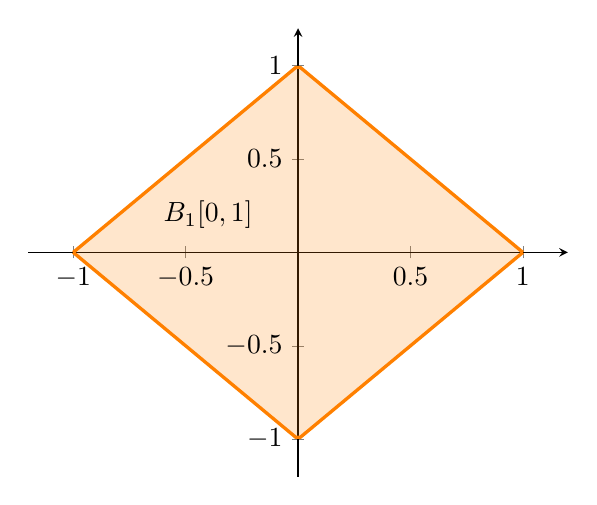
\begin{tikzpicture}
      \begin{axis}[
          axis lines=middle,
          xmax = 1.2,
          xmin = -1.2,
          ymax = 1.2,
          ymin = -1.2,]
        \addplot [
          domain=-1:1,
          samples=100,
          name path=upper,
          very thick, orange]{1 - abs(x)};
        \addplot [
          domain=-1:1,
          samples=100,
          name path=lower,
          very thick, orange]{abs(x) - 1};
        \addplot [
          thick,
          color=orange,
          fill=orange,
          fill opacity=0.2
        ]
        fill between[
          of=upper and lower,
          soft clip={domain=-1:1},
        ];
        \node at (-.4,.2) {$B_1[0,1]$};
      \end{axis}
    \end{tikzpicture}

  \item $B_2[0, 1] = \qty{x \in \mathbb{R}^2 | (x_1)^2 + (x_2)^2 \leq 1}$

    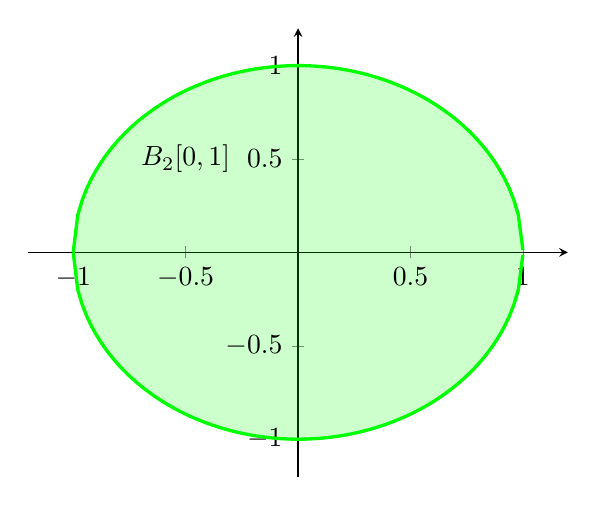
\begin{tikzpicture}
      \begin{axis}[
          axis lines=middle,
          xmax = 1.2,
          xmin = -1.2,
          ymax = 1.2,
          ymin = -1.2,]
        \addplot [
          domain=-1:1,
          samples=100,
          name path=upper,
          very thick, green]{sqrt(1 - x^2)};
        \addplot [
          domain=-1:1,
          samples=100,
          name path=lower,
          very thick, green]{-sqrt(1 - x^2)};
        \addplot [
          thick,
          color=green,
          fill=green,
          fill opacity=0.2
        ]
        fill between[
          of=upper and lower,
          soft clip={domain=-1:1},
        ];
        \node at (-.5,.5) {$B_2[0,1]$};
      \end{axis}
    \end{tikzpicture}

  \newpage
  \item $B_{\infty}[0, 1] = \qty{x \in \mathbb{R}^2 | \max\qty{\abs{x_1}, \abs{x_2}} \leq 1}$

      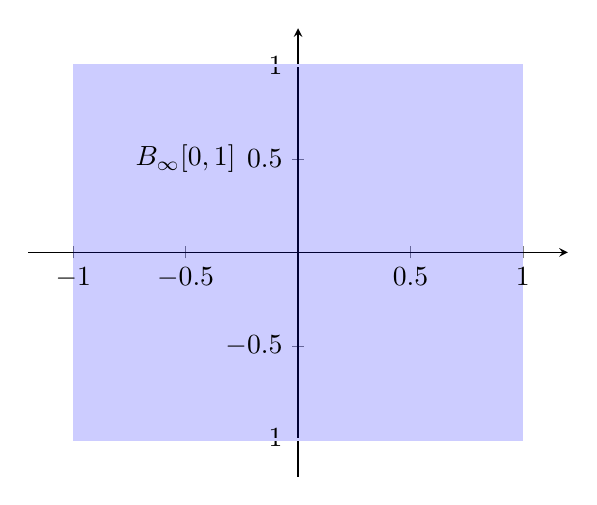
\begin{tikzpicture}
        \begin{axis}[
            axis lines=middle,
            xmax = 1.2,
            xmin = -1.2,
            ymax = 1.2,
            ymin = -1.2,]
          \addplot [
            domain=-1:1,
            samples=100,
            name path=upper,
            very thick, blue!20]{1};
          \addplot [
            domain=-1:1,
            samples=100,
            name path=lower,
            very thick, blue!20]{-1};
          \addplot [
            thick,
            color=blue,
            fill=blue,
            fill opacity=0.2
          ]
          fill between[
            of=upper and lower,
            soft clip={domain=-1:1},
          ];
          \node at (-.5,.5) {$B_{\infty}[0,1]$};
        \end{axis}
      \end{tikzpicture}
    \end{itemize}

    Bei der Betrachtung der Bilder fällt auf, dass
    \[\begin{aligned}
      B_{\infty}[0,1]   & \geq & B_2[0,1]   & \geq & B_1[0,1] \\
      \norm{x}_{\infty} & \leq & \norm{x}_2 & \leq & \norm{x}_1
    \end{aligned}\]

  \item
    Für $x = 0$ ist alles klar.
    Sei $x \ne 0 \Rightarrow \frac{\abs{x_k}}{\norm{x}_q} \leq 1$ für $k = 1, \ldots, N$.
    Weiter ist $p \mapsto t^p$ für $t \in [0, 1]$ auf $[1, +\infty)$ monoton fallend.
    \begin{align*}
      \overset{q > p}&\Rightarrow \qty(\frac{\abs{x_k}}{\norm{x}_q})^q \leq \qty(\frac{\abs{x_k}}{\norm{x}_q})^p \\
                     &\Rightarrow \sum_{k = 1}^N \frac{\abs{x_k}^q}{\norm{x}_q^q}
                       = \frac{1}{\norm{x}_q^q} \underset{= \norm{x}_q^q}{\underbrace{\sum_{k = 1}^N \abs{x_k}^q}}
                       = 1 \leq \sum_{k = 1}^N \frac{\abs{x_k}^p}{\norm{x}_q^p} = \qty(\frac{\norm{x}_p}{\norm{x}_q})^p
                     && {\Big |} \quad (\ldots)^{\sfrac{1}{p}} \\
                     &\Rightarrow \colorbox{green!20}{$1 \leq \frac{\norm{x}_p}{\norm{x}_q}$}
    \end{align*}
    Für $p = \infty$ existiert ein $k_0$ mit $\abs{x_{k_0}} = \norm{x}_{\infty} = \max\qty{\abs{x_1}, \ldots, \abs{x_N}}$

    \begin{align*}
      \Rightarrow \abs{x_{k_0}}
        &= \colorbox{orange!50}{$\norm{x}_{\infty}$} = \qty\Big(\abs{x_{k_0}}^p)^{\sfrac{1}{p}}
          \leq \qty(\sum_{k = 1}^N \abs{x_k}^p)^{\sfrac{1}{p}} = \norm{x}_p \\
        &\leq \sum_{k = 1}^N \qty\Big(\abs{x_{k_0}}^p)^{\sfrac{1}{p}}
          = N^{\sfrac{1}{p}} \abs{x_{k_0}} =\colorbox{purple!50}{$N^{\sfrac{1}{p}} \norm{x}_{\infty}$}
    \end{align*}

  \end{enumerate}

\section{Blatt 03 - Hausaufgabe 3}
\begin{enumerate}[a)]
\item $d$ definiert eine Metrik auf $M \times M$, wenn
  \begin{itemize}
  \item $\forall x, y \in M \colon d(x,y) \geq 0$ und
    $\forall x,y \in M \colon d(x,y) = 0 \iff x = y$

    Diese Bedingung ist durch die Definition von $d$ erfüllt.

  \item $\forall x,y \in M \colon d(x, y) = d(x, y)$
    \begin{enumerate}[label={Fall \arabic*:},leftmargin=*]
    \item $x \ne y \colon d(x, y) = 1 = d(y, x)$
    \item $x = y \colon d(x, y) = 0 = d(y, x)$
    \end{enumerate}

  \item $\forall x,y,z \in M \colon d(x,y) \leq d(x,z) + d(y,z)$
    \begin{enumerate}[label={Fall \arabic*:},leftmargin=*]
    \item $x \ne y \land x \ne z \land y \ne z \colon d(x, y) = 1 \leq d(x, z) + d(y, z) = 2$
    \item $x = y \land x = z \land y = z \colon d(x, y) = 0 \leq d(x, z) + d(y, z) = 0$
    \item $x \ne y \land y = z \colon d(x, y) = 1 \leq d(x, z) + d(y, z) = 1$
    \item $x = y \land x \ne z \colon d(x, y) = 0 \leq d(x, z) + d(y, z) = 2$
    \end{enumerate}

  \end{itemize}

\item
  \begin{enumerate}[label={Fall \arabic*:},leftmargin=*]
  \item $0 < r < 1$

    $d(x, y) < r$ wenn $y = x$

    $\Rightarrow$ Kugeln entsprechen $\qty{x}$
  \item $r = 1$

    $B(x, r) = \qty{x}$ und $B[x,r] = M$
  \item $r > 1$

    $B(x, r) = B[x, r] = M$
  \end{enumerate}
\end{enumerate}

\section{Blatt 04 - Aufgabe 3}

\textit{Lsg.} Sei $(M, d)$ ein metrischer Raum und $A \subseteq M$.

\begin{itemize}
\item $x \in \mathring A = \text{int} A \iff \exists r > 0 \colon B(x, r) \subseteq A$
\item $\mathring A$ ist die größte offene Teilmenge von $A$.
  $A \subseteq M$ heißt offen, falls $A = \mathring A$ gilt.

  $x \in \partial A \iff x \in \overline A \setminus \mathring A
  \iff \forall r > 0 \colon B(x, r) \cap A \ne \emptyset \land B(x, r) \cap (M \setminus A) \ne \emptyset$

  $\partial A = \partial (M \setminus A)$
\item $A \subseteq M$ heißt abgeschlossen $\iff M \setminus A$ ist offen.
  $\overline A$ Abschluss von $A \colon$ kleinste abgeschlossene Menge von $A$

  $x \in \overline A \iff \forall r > 0 \colon B(x, r) \cap A \ne \emptyset$

  Es gibt eine Folge $\qty(x_n)$ in $A$ mit $x_n \to x$
\end{itemize}

$x$ ist isolierter Punkt von $A \iff \exists r > 0 \colon B(x, r) \cap A = \qty{x})$

\begin{enumerate}[(i)]
\item $A = B(x, r)$ mit $x \in \mathbb{R}^2$ und $r > 0$

  \textit{Lsg.} $A = \mathring A \colon $ Sei $y \in B(x, r) \Rightarrow \epsilon = r - \norm{x - y}_2 > 0$

  Zu zeigen ist nun, dass $y \in \mathring A$:

  Es gilt $B(y, \epsilon) \subseteq B(x, r) \colon$ Sei $z \in B(y, \epsilon)$

  $\Rightarrow \norm{x - z}_2 \leq \norm{x - y}_2 + \underset{< \epsilon}{\underbrace{\norm{y - z}_2}}
  < \norm{x - y}_2 + (r - \norm{x - y}_2) = r$

  $\Rightarrow z \in B(x, r) \Rightarrow$ die Menge ist offen.

  Es gilt $\partial A = S(x, r) = \qty{ y \in \mathbb{R}^2 \middle| \norm{x - y}_2 = r }$

  Ist $\norm{x - y} > r$, dann existiert ein $\epsilon > 0$ mit
  $B(y, \epsilon) \subseteq \mathbb{R}_2 \setminus A$

  $\Rightarrow y$ ist kein Randpunkt von $A$ und gehört nicht zu $\mathring A$.

  $A = \mathring A \cup \partial A = B[x, r]$
\item $A = B[x, r] = \qty{y \in \mathbb{R}^2 \middle| \norm{x - y}_2 \leq r}$ mit $x \in \mathbb{R}^2$ und $r > 0$

  \textit{Lsg.} $A$ ist eine abgeschlossene Kugel, da $\overline A = A$ gilt.

  Weiter ist $\mathring A = B(x, r)$ und $\partial A = S(x, r)$

\item $A = \qty{y \in \mathbb{R}^2 \middle| \norm{x - y}_2 > r}$ mit $x \in \mathbb{R}^2$ und $r > 0$

  \textit{Lsg.} $A$ ist offen (da $\mathbb{R}^2$ ohne abgeschlossene Kugel), d.h. $A = \mathring A$

  $\partial A = \partial B[x, r] = S(x, r)$

  $\overline A = \qty{y \in \mathbb{R}^2 \middle| \norm{x - y}_2 \geq r}$

\item $A = \qty{x = \qty(x_1, x_2) \in \mathbb{R}^2 \middle| \qty(x_1 > -1) \land \qty(x_2 \geq -1)}$

  \textit{Lsg.}:

  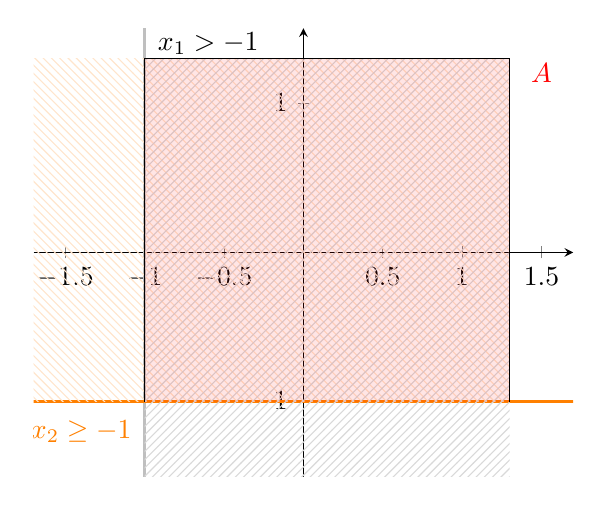
\begin{tikzpicture}
    \begin{axis}[
      axis lines=middle,
      xmax = 1.7,
      xmin = -1.7,
      ymax = 1.5,
      ymin = -1.5,]
      \addplot [
        name path=f,
        very thick,
        gray!50] coordinates {(-1,-2) (-1, 2)};
      \addplot [
        name path=g,
        domain=-2:2,
        samples=100,
        very thick, orange]{-1};
      \addplot[draw=none, pattern color=orange!20, pattern=north west lines] coordinates
        {(-2, 1.3) (1.3, 1.3) (1.3, -1) (-2, -1)};
      \addplot[draw=none, pattern color=gray!30, pattern=north east lines] coordinates
        {(-1, 1.3) (1.3, 1.3) (1.3, -2) (-1, -2)};
      \node[orange] at (-1.4, -1.2) {$x_2 \geq -1$};
      \node at (-0.6, 1.4) {$x_1 > -1$};
      \node[red] at (1.5, 1.2) {$A$};
      \addplot[fill=red, fill opacity=.1] coordinates {(-1,-1) (-1,1.3) (1.3,1.3) (1.3,-1)};
    \end{axis}
  \end{tikzpicture}

  $\mathring A = \qty{x = \qty(x_1, x_2) \middle| x_1 > -1 \land x_2 > -1 }$ (eine echte Teilmenge von $A$).

  $\partial A = \qty{ (-1, x_2), (x_1, -1) \middle| x_1, x_2 \geq 0 }$

  $\overline A = \mathring A \cup \partial A = \qty{x \in \mathbb{R}^2 \middle| x_1 \geq 0 \land x_2 \geq 0}$
  (eine echte Unmenge zu $A \Rightarrow A$ ist nicht abgeschlossen)

\item $A = \qty{ x_n = \qty(\frac{1}{n}, 0) \middle| n \in \mathbb{N}}$

  \textit{Lsg.}

    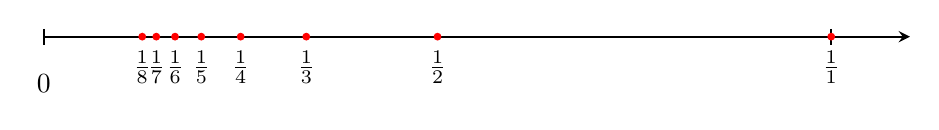
\begin{tikzpicture}
      \draw[-stealth, thick] (0,0) -> (11,0);
      \draw[thick] (0,.1) -- ++(0,-.2);
      \draw[thick] (10,.1) -- ++(0,-.2);
      \node at (0, -.6) {0};
      \foreach \x [evaluate=\x as \xx using (10/\x)]in {1,...,8} {
        \node[circle, fill=red, inner sep=1pt, label=below:$\frac{1}{\x}$] at (\xx, 0) {};
      }
  \end{tikzpicture}

  $\mathring A = \emptyset, \partial A = A \cup \qty{(0, 0)} \supsetneqq A$ wegen $\lim_{n \to \infty} x_n = 0$

  $\Rightarrow A$ ist weder offen noch abgeschlossen.

  Alle Punkte aus $A$ sind isoliert.
\end{enumerate}

\section{Blatt 04 - Aufgabe 4}

Sei $(X, d)$ ein metrischer Raum und $M \subseteq X$ eine nichtleere Teilmenge von $X$.

$d_M \colon M \times M \to \mathbb{R}$ mit $d_m(x, y) \coloneqq d(x, y) \quad x, y \in M$
auf $M$ induzierte Metrik.

\begin{align*}
  B_d(x, r) &= \qty{ y \in X \middle| d(x, y) < r } \\
  B_{d_M}(x, r) &= \qty{ y \in M \middle| d_M(x, y) = d(x, y) < r } \\
            &= B_d(x, r) \cap M
\end{align*}

($A \subseteq M$ ist $d_M$-abgeschlossen $\iff \exists B \subseteq X$, die $d$-abgeschlossen ist, mit $A = B \cap M$)

$(R, d), d(x, y) = \abs{x - y}$

\begin{enumerate}[a)]
\item Geben Sie die Mengen $B_d\qty(\frac{3}{2}, r)$ und $B_{d_M}\qty(\frac{3}{2}, r)$
  für $r = 1$ bzw. $r = \frac{1}{2}$ an.

  \textit{Lsg.} $B_d\qty(\frac{3}{2}, 1) = \qty(\frac{3}{2} - 1, \frac{3}{2} + 1) = \qty(\frac{1}{2}, \frac{5}{2})$

  $B_{d_M}\qty(\frac{3}{2}, 1) = B_d\qty(\frac{3}{2}, 1) \cap M = \left(\frac{1}{2}, 1\right] \cup \qty{\frac{3}{2}} \cup \qty(2, \frac{5}{2})$

  $B_d\qty(\frac{3}{2}, \frac{1}{2}) = \qty(\frac{3}{2} - \frac{1}{2}, \frac{3}{2} + \frac{1}{2}) = \qty(1, 2)$

  $B_{d_M}\qty(\frac{3}{2}, \frac{1}{2}) = B_d\qty(\frac{3}{2}, \frac{1}{2}) \cap M = \qty{\frac{3}{2}}$

\item Welche der folgenden Mengen $A_k$ sind offen/abgeschlossen in den Räumen $(\mathbb{R}, d)$
  bzw. $(M, d_M)$, wobei $A_1 = [0, 1)$, $A_2 = [0, 1) \cup \qty{\frac{3}{2}}$, $A_3 = (2, 3)$,
  $A_4 = M$ gilt?

  \textit{Lsg.}
  $B_{d_M}\qty(\frac{3}{2}, 0) = \left[0, \frac{1}{2}\right) \colorbox{green}{$\subseteq A_1$}$ ist offen in $\qty(M, d_M)$

  \begin{enumerate}[label={$A_{\arabic*}$}]
  \item $= [0, 1)$ ist in $(\mathbb{R}, d)$ weder offen noch abgeschlossen.
  \item $= [0, 1) \cup \qty{\frac{3}{2}}$ ist in $(\mathbb{R}, d)$ weder offen noch abgeschlossen.
  \item $= (2, 3)$ ist in $(\mathbb{R}, d)$ offen aber nicht abgeschlossen.
  \item $= M$ ist in $(\mathbb{R}, d)$ weder offen noch abgeschlossen.
  \end{enumerate}
  \begin{enumerate}[label={$A_{\arabic*}$}]
  \item $= [0, 1)$ ist in $(M, d_M)$ \colorbox{green}{offen} und abgeschlossen.
  \item $= [0, 1) \cup \qty{\frac{3}{2}}$ ist in $(M, d_M)$ offen und abgeschlossen.
  \item $= (2, 3)$ ist in $(M, d_M)$ offen und abgeschlossen.
  \item $= M$ ist in $(M, d_M)$ offen und abgeschlossen.
  \end{enumerate}

\item Ist $\qty(M, d_M)$ ein vollständiger metrischer Raum?

  \textit{Lsg.} Sei $x_n \coloneqq 1 - \frac{1}{n} \in M$

  $\Rightarrow \qty(x_n)$ ist in $(\mathbb{R}, d)$ eine konvergente Folge mit
  $\lim_{n \to \infty} x_n = 1 \Rightarrow \qty(x_n)$ ist eine Cauchy-Folge in
  $(\mathbb{R}, d)$ und $\qty(M, d_M)$.

  Wegen $1 \notin M$ ist $\qty(x_n)$ nicht konvergent in $\qty(M, d_M)$
  und somit ist $\qty(M, d_M)$ nicht vollständig.
\end{enumerate}

\section{Blatt 04 - Hausaufgabe 1}

Das Innere von $\mathbb{Q}$, die Menge $\mathring{\mathbb{Q}}$ ist definiert als die Vereinigung aller
offenen Teilmengen von $\mathbb{Q}$.
Eine Teilmenge $A \subseteq \mathbb{Q}$ heißt offen, wenn es ein Element $q \in \mathbb{Q}$
und ein $r > 0$ gibt, so dass $B(x, r) \subseteq A$.
Nun sind $q, q + r \in \mathbb{R}, q < q + r$.
Damit ist $(q, q + r) \setminus \mathbb{Q} \ne \emptyset$, denn zwischen zwei reellen Zahlen liegt
immer mindestens eine irrationale Zahl (Korollar 1.4.9 der Vorlesung).
Somit existiert keine offene Teilmenge $A \subseteq \mathbb{Q}, A \ne \emptyset$.

Damit ist $\mathring{\mathbb{Q}} = \emptyset$. \\

Der Abschluß von $\mathbb{Q}$, die Menge $\overline{\mathbb{Q}}$ ist definiert als
die Schnittmenge aller abgeschlossenen Teilmengen von $\mathbb{R}$, die $\mathbb{Q}$
enthalten.

Sei $A$ eine abgeschlossene, echte Teilmenge von $\mathbb{R}$, die $\mathbb{Q}$ enthält.
Damit $A$ abgeschlossen ist, muss das Komplement von $A$, die Menge $\mathbb{R} \setminus A$
offen sein, das heißt für jedes $x \in A$ existiert ein $r > 0$ mit $B(x, r) \subseteq A$.
Nun sind $x, x + r \in \mathbb{R}, x < x + r$.
Damit ist $(q, q + r) \cap \mathbb{Q} \ne \emptyset$, denn zwischen zwei reellen Zahlen liegt
immer mindestens eine rationale Zahl (Korollar 1.4.9 der Vorlesung).
Das ist ein Widerspruch dazu, dass $\mathbb{Q} \subseteq A$.
Somit existiert keine abgeschlossene, echte Teilmenge von $\mathbb{R}$, die $\mathbb{Q}$ enthält.
Damit ist die Schnittmenge aller abgeschlossenen Teilmengen von $\mathbb{R}$, die $\mathbb{Q}$
enthalten gleich $\mathbb{R} = \overline{\mathbb{Q}}$.

Der Rand von $\mathbb{Q}$, die Menge $\partial \mathbb{Q}$ ist definiert als
$\overline{\mathbb{Q}} \setminus \mathring{\mathbb{Q}} = \mathbb{R} \setminus \emptyset = \mathbb{R}$.

\section{Blatt 04 - Hausaufgabe 3}

\begin{enumerate}[(i)]
\item Beweisen Sie, dass $(M, d)$ ein metrischer Raum ist.

  \textit{Lsg.} $(M, d)$ ist ein metrischer Raum, falls die Abbildung $d$ folgende 3 Eigenschaften
  erfüllt:
  \begin{enumerate}[(i)]
  \item $\forall x, y \in M \colon d(x, y) \geq 0$ und $d(x, y) = 0 \iff x = f$

    Der erste Teil der Eigenschaft ist durch die Definition des Betrags erfüllt.
    Weiterhin  gilt $\abs{\ln x - \ln y} = 0 \iff \ln x = \ln y \iff x = y$,
    da $\ln$ monoton steigend und somit injektiv ist.

  \item \textbf{Symmetrie}. $\forall x, y \in M \colon d(x, y) = d(y, x)$

    Diese Eigenschaft ist erfüllt, da
    \[
      \abs{\ln x - \ln y} = \abs{-1 \cdot (\ln y - \ln x)} = \abs{\ln y - \ln x}
    \]

  \item \textbf{Dreiecksungleichung}. $\forall x, y, z \in M \colon d(x, y) \leq d(x, z) + d(z, y)$

    Diese Eigenschaft ist erfüllt, da
    \begin{align*}
      d(x, y) &= \abs{\ln x - \ln y} \\
              &= \abs{\ln x + 0 - \ln y} \\
              &= \abs{\ln x - \ln z + \ln z -  \ln y} \\
              &\leq \abs{\ln x - \ln z} + \abs{\ln z - \ln y} \\
              &= d(x, z) + d(z, y)
    \end{align*}
  \end{enumerate}

\item Sei $d|_M$ die von $(\mathbb{R}, \abs{\cdot})$ induzierte Metrik auf $M$.
  Untersuchen Sie, ob die Räume $(M, d)$ und $\qty(M, d|_M)$ vollständig sind. \\

  \textit{Lsg.} $d|_M \colon M \times M \to \mathbb{R}, d|_m(x, y) = \abs{x - y}$.

  Sei $a_n \coloneqq \frac{1}{n} \in M$.
  Dann ist $\qty(a_n)$ in $(\mathbb{R}, \abs{\cdot})$ eine konvergente Folge mit
  $\lim_{n \to \infty} a_n = 0$.
  Damit ist $\qty(a_n)$ eine Cachy-Folge in $(\mathbb{R}, \abs{\cdot})$ und $(M, d|_M)$.

  Wegen $0 \notin M$ ist $\qty(a_n)$ nicht konvergent in $(M, d|_M)$ und somit ist $(M, d|_M)$
  nicht vollständig. \\

  Sei $\qty(b_n)$ eine Cauchy-Folge in $(M, d)$.
  Sei $e^r$ so, dass
  \[
    \forall \epsilon > 0 \exists n_0 \in \mathbb{N} \forall n \in \mathbb{N}_{\geq n_0} \colon
    \abs{\ln b_n - \ln e^r} = \abs{\ln b_n - r} < \epsilon
  \]
  Da $\qty(b_n)$ eine Cauchy-Folge ist, gilt $\ln b_n \in \mathbb{R}$ somit ist auch $r \in \mathbb{R}$
  und $e^r \in M$.
  Damit konvergieren alle Cauchy-Folgen in $\qty(M, d)$ gegen einen Wert in $M$ und $\qty(M, d)$
  ist vollständig.

\end{enumerate}

\section{Blatt 04 - Hausaufgabe 4}

\begin{enumerate}[(i)]
\item Für ein $q \in (0, 1)$ und $f(x) = 1 + qx$ sei
  $x_n = \qty(f^n(q), f^n(1), f^n(1 + q)) \in \mathbb{R}^3$, hierbei bezeichne
  $f^n = \underset{n-\text{mal}}{\underbrace{f \circ \ldots \circ f}}$ die $n$-fache
  Anwendung der Funktion $f$. \\

  \textit{Lsg.} Bestimmung einer expliziten Darstellung von $f^n(x)$

  \textit{Behauptung:} $P(n) \colon f^n (x) = \qty(\sum_{k = 0}^{n - 1} q^k) + q^nx$ \\
  \textit{Induktionsanfang}: $P(1) \colon f^1(x) = \qty(\sum_{k = 0}^{0} q^k) + q^1x = 1 + qx$ \\
  \textit{Induktionsschritt}: $P(n + 1) \colon f^{n + 1} = \qty(\sum_{k = 0}^{n} q^k) + q^{n + 1}x
  = 1 + q\qty(\qty(\sum_{k = 0}^{n - 1} q^k) + q^{n}x) = f(f^{n - 1}(x))$.
  \begin{align*}
    x_n = \qty(\frac{q^n - 1}{q - 1} + q^{n + 1}, \frac{q^{n + 1} - 1}{q - 1}, \frac{q^{n + 2} - 1}{q - 1})
  \end{align*}
  Die Folgen $\qty(\frac{q^n - 1}{q - 1} + q^{n + 1})_{n \in \mathbb{N}}$,
  $\qty(\frac{q^{n + 1} - 1}{q - 1})_{n \in \mathbb{N}}$
  und
  $\qty(\frac{q^{n + 2} - 1}{q - 1})_{n \in \mathbb{N}}$ sind konvergente Folgen aus
  $\mathbb{R}$ mit $\lim_{m \to \infty} (\ldots) = \frac{1}{1 - q}$.
  Folglich ist auch $(x_n)$ beschränkt mit
  $\lim_{n \to \infty} x_n = \qty( \frac{1}{1 - q},  \frac{1}{1 - q},  \frac{1}{1 - q}) \in \mathbb{R}^3$.
\item Für eine Nullfolge $\qty(y_n)$ aus $\mathbb{R}$ sei
  $x_n = \qty(y_n, y_{2n}^2, y_{3n}^n) \in \mathbb{R}^3$.

  \textit{Lsg.} $\qty(y_n)$ ist eine Nullfolge aus $\mathbb{R}$.
  Somit sind auch $\qty(y_{2n})$ und $\qty(y_{3n})$ Nullfolgen.
  Aus Proposition 2.1.5 (b) der Vorlesung folgt, dass auch $y_{2n}^2$ und $y_{3n}^n$ Mullfolgen sind.

  Folglich ist auch $\qty(x_n)$ beschränkt mit $\lim_{n \to \infty} x_n = 0$
\end{enumerate}

\section{Blatt 05 - Aufgabe 2}

\begin{enumerate}[a)]
\item Zeigen Sie, dass die Funktion $f$ partiell stetig auf $\mathbb{R}^2$ ist,
  dass heißt für jeden Punkt $x = (x_1, x_2) \in \mathbb{R}^2$ sind die
  Abbildungen $g_1(t) \coloneqq f(x_1 + t, x_2)$ und
  $g_2(t) \coloneqq f(x_1, x_2 + t)$ stetig in $t = 0$.
\item Zeigen Sie, dass die Funktion $f$ nicht stetig auf $\mathbb{R}^2$ ist.

  \textit{Lsg.} Die Funktion ist nicht stetig im Punkt $x = (0, 0)$.

  Falls die Funktion $f$ in $x$ stetig wäre, müsste gelten:
  \[
    \lim_{t \to 0} f(t, t) = f(0, 0)
  \]
  Nun ist jedoch $f(0, 0) = 0$ und
  $\lim_{t \to 0} f(t, t) = \lim_{t \to 0} \frac{t^2}{2t^2} = \frac{1}{2}$.
  Ein Widerspruch, damit ist $f$ auf $\mathbb{R}^2$ nicht stetig.
\end{enumerate}

\section{Blatt 05 - Hausaufgabe 2}

Untersuchen Sie die Funktionen $f \colon \mathbb{R}^2 \to \mathbb{R}$ definiert
durch
\[
  f(x, y) = \begin{cases}
    \frac{\sin(xy)}{x} & \text{für } x \ne 0 \\
    y & \text{für } x = 0 \\
  \end{cases}
\]
auf Stetigkeit. \\

\textit{Lsg.}
\begin{center}
  \resizebox{.8\textwidth}{!}{
    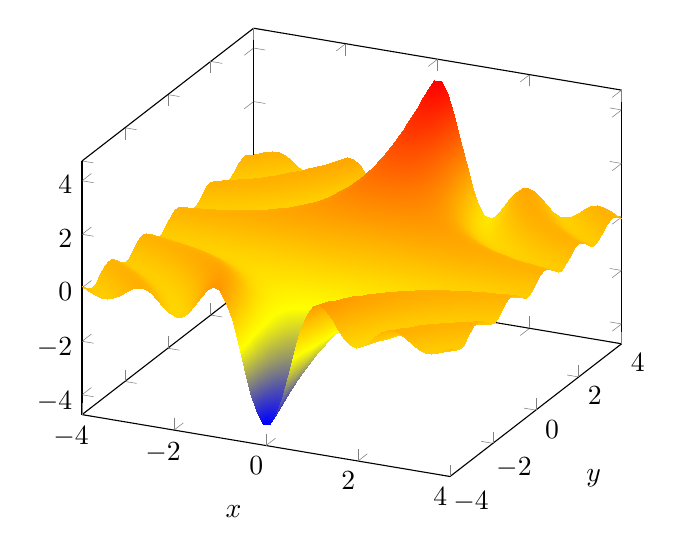
\begin{tikzpicture}[
      declare function={
        f(\x, \y) = \x != 0 ? sin(deg(\x * \y))/\x : \y;
      }
    ]
      \begin{axis}[
        xlabel = $x$,
        ylabel = $y$
      ]
        \addplot3[
          surf,
          domain=-4:4,
          samples=60,
          shader=interp,
        ] {f(x, y)};
      \end{axis}
    \end{tikzpicture}
  }
\end{center}

Seien $(\mathbb{R}^2, \norm{\cdot}_2)$ und $(\mathbb{R}, \abs{\cdot})$
metrische Räume. \textbf{Vorüberlegungen}
\[
  \text{Für ein $y \in \mathbb{R}$ ist $\sin(xy)$ periodisch und $\sup\qty(\frac{\sin(xy)}{x}) = $ }
  \lim_{x \to 0} \frac{\sin(xy)}{x} = y
\]

\textbf{Annahme}: $f$ ist Lipschtzstetig.
\begin{align*}
  \exists L \geq 0 \forall (x_1, y_1), (x_2, y_2) \in \mathbb{R}^2 \colon d_2(f(x_1, y_1), f(x_2, y_2))
    &\leq L d_1((x_1, y_1), (x_2, y_2)) \\
  \abs{\frac{\sin(x_1y_1)}{x_1} - \frac{\sin(x_2y_2)}{x_2}}
    &\leq L \sqrt{(x_1 - x_2)^2 + (y_1 - y_2)^2} \\
  \abs{\frac{\sin(x_1y_1)}{x_1} - \frac{\sin(x_2y_2)}{x_2}}
    \leq \abs{y_1 - y_2} &\leq L \cdot \abs{y_1 - y_2}
    \leq L\sqrt{(x_1 - x_2)^2 + (y_1 - y_2)^2} \\
  \frac{\abs{y_1 - y_2}}{\abs{y_1 - y_2}} &\leq L \\
  1 &\leq L \\
  \Rightarrow f \text{ ist Lipschitzstetig}
\end{align*}

\section{Blatt 06 - Aufgabe 1}

Skizzieren Sie die folgenden Mengen $K \in \mathbb{R}^2$.
Untersuchen Sie, ob die angegebenen Funktionen $f: K \to \mathbb{R}$
Minimum und Maximum auf $K$ besitzen.
\begin{enumerate}[(i)]
\item $K \coloneqq \qty{x = \qty(x_1, x_2) \in \mathbb{R}^2 \middle|
    (x_1, x_2 \geq 0) \land (2x_1 + x_2 \leq 3)}$ und
  $f\qty(x_1, x_2) \coloneqq \sin\qty(x_1 \cdot x_2) \cdot
  \ln\qty(\frac{1 + x_1}{2 + x_2^2})$

  \textit{Lsg.} Aus den Beschränkungen für $x_1$ und $x_2$ folgt
  \[
    0 \leq x_1 \leq \frac{1}{2}\qty(3- x_2) \leq \frac{3}{2}
    \text{ und }
    0 \leq x_2 \leq 3 - 2x_1 \leq 3
  \]
  $\Rightarrow K \subseteq A \coloneqq [0, 3] \times [0, 3]
  \Rightarrow K$ ist beschränkt.

  \begin{center}
    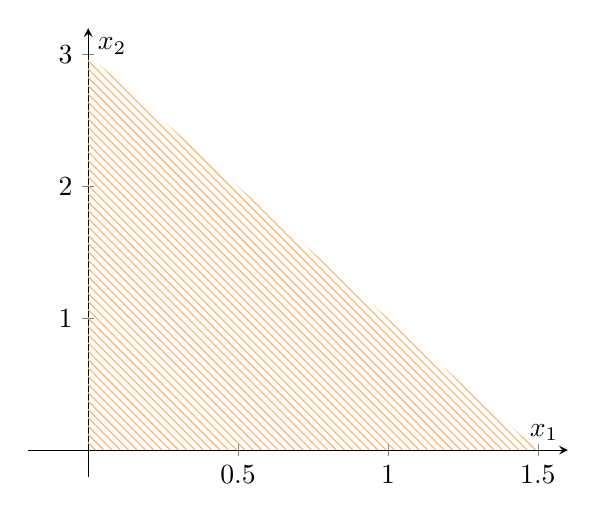
\begin{tikzpicture}
      \begin{axis}[
        axis lines=middle,
        xlabel=$x_1$,
        xmax = 1.6,
        xmin = -0.2,
        ylabel=$x_2$,
        ymax = 3.2,
        ymin = -0.2,
      ]
        \addplot[draw=none, pattern color=orange!60, pattern=north west lines] coordinates
        {(0, 0) (0, 3) (1.5, 0)};
      \end{axis}
    \end{tikzpicture}
  \end{center}
  Die Funktionen $g(x_1, x_2) \coloneqq x_1$, $h(x_1, x_2) \coloneqq x_2$,
  $j(x_1, x_2) \coloneqq 2x_1 + x_2$ sind stetig.

  Die Urbilder abgeschlossener Mengen
  \begin{flalign*}
    A_1 &= g^{-1}([0, \infty)) = [0, \infty) \times \mathbb{R} & \\
    A_2 &= h^{-1}([0, \infty)) = \mathbb{R} \times [0, \infty) \\
    A_3 &= j^{-1}((-\infty, 3]) = \qty{(x_1, x_2) \in \mathbb{R}^2 \middle|
      (x_1 \in \mathbb{R}) \land (x_2 \leq 3 - 2x_1)}
  \end{flalign*}
  sind somit abgeschlossen und
  $K = A_1 \cap A_2 \cap A_3$ ist ebenfalls abgeschlossen.
  Weiterhin ist $f$ als Komposition stetiger Funktionen ebenfalls stetig
  und es existieren Punkte $a = (a_1, a_2), b = (b_1, b_2) \in \mathbb{R}^2$
  mit $f(a) \leq f(x) \leq f(b) \forall x \in K$.

\item $K \coloneqq \qty{x = \qty(x_1, x_2) \in \mathbb{R}^2 \middle|
    \abs{x_1 \cdot x_2} \leq 1}$ und
  $f\qty(x_1, x_2) \coloneqq \sin(x_1) + \abs{x_2}$ \\

  \textit{Lsg.}
  \begin{flalign*}
    K &= \qty{(x_1, x_2) \in \mathbb{R}^2 \middle|
         x_1 = 0 \lor x_2 \leq \frac{1}{\abs{x_1}}} & \\
      &= \qty(\bigcup_{x_1 \ne 0} \qty{x_1} \times
         \qty[-\frac{1}{\abs{x_1}}, \frac{1}{\abs{x_1}}])
         \cup \qty{\qty{0} \times \mathbb{R}}
   \end{flalign*}
   $\Rightarrow K$ ist nicht beschränkt $K$ ist nicht kompakt.

   \begin{center}
     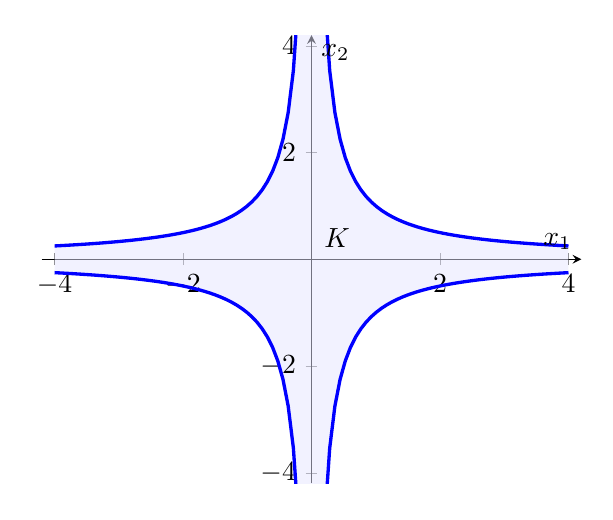
\begin{tikzpicture}[
         declare function={
           f(\x) = \x != 0 ? 1 / abs(\x) : 5;
         }
       ]
       \begin{axis}[
         axis lines=middle,
         xlabel=$x_1$,
         xmax = 4.2,
         xmin = -4.2,
         ylabel=$x_2$,
         ymax = 4.2,
         ymin = -4.2,
       ]
         \addplot[
           domain = -4:4,
           very thick,
           name path = f1,
           samples = 100,
           blue,
         ] {f(x)};
         \addplot[
           domain = -4:4,
           very thick,
           name path = f2,
           samples = 100,
           blue,
         ] { -1 *  f(x)};
         \addplot[
           fill = blue!10,
           fill opacity = .5,
         ] fill between[of = f1 and f2];
         \node at (.4,.4) {$K$};
       \end{axis}
     \end{tikzpicture}
   \end{center}

   Auch $f$ ist wegen $f(0, x_2) = \abs{x_2}, x_2 \in \mathbb{R}$
   nicht nach oben beschränkt.
   $\Rightarrow f$ besitzt kein Maximum oder Supremum auf $K$.

  \begin{minipage}[t]{.45\textwidth}
    \textbf{Fall 1}: $x_1 = 0$:
    \[
      f(x_1, x_2) = \abs{x_2} \geq 0, x_2 \in \mathbb{R}
    \]
  \end{minipage}
  \vrule
  \hfill
  \begin{minipage}[t]{.45\textwidth}
    \textbf{Fall 2}: $x_2 = 0$
    \begin{align*}
      f{x_1, x_2} &= \sin(x_1) + \abs{x_2} \geq \sin(x_1) \\
                  &= f(x_1, 0) \geq -1 \\
                  &= f\qty(2k\pi + \frac{3}{2}\pi, 0), k \in \mathbb{Z}
    \end{align*}
  \end{minipage} \\

  $f$ besitzt auf $K$ das Minimum $-1$
\end{enumerate}

\section{Blatt 06 - Hausaufgabe 1}

Aus den Beschränkungen für $x_1$ und $x_2$ folgt
\[
  0 \leq x_1 \leq 4 \text{ und } 2 - \sqrt{2} \leq x_2 \leq 2 + \sqrt{2}
\]
$\Rightarrow K \subseteq [0, 4] \times [0, 4] \Rightarrow K$ ist beschränkt.

\begin{center}
  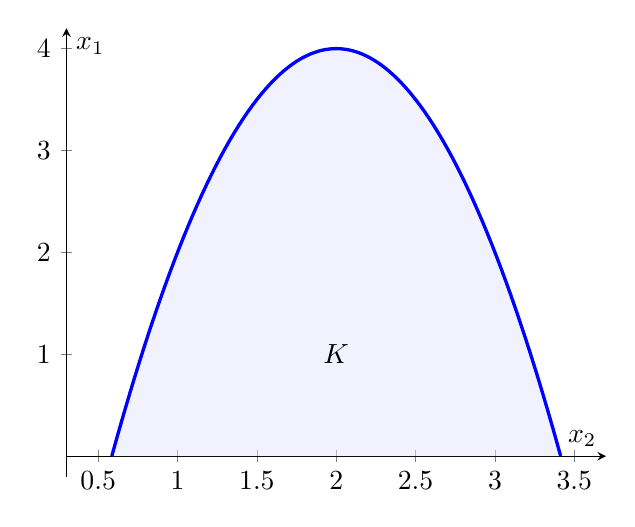
\begin{tikzpicture}[
      declare function={
        f(\x) = 2 * (2 - (\x - 2)^2);
      }
    ]
    \begin{axis}[
      axis lines=middle,
      xlabel=$x_2$,
      xmax = 3.7,
      xmin = 0.3,
      ylabel=$x_1$,
      ymax = 4.2,
      ymin = -0.2,
      ]
      \path[name path=axisa] (axis cs:0.586,0) -- (axis cs:3.414,0);
      \addplot[
        domain = 0.586:3.414,
        very thick,
        name path = f1,
        samples = 100,
        blue,
      ] {f(x)};
      \addplot[
        fill = blue!10,
        fill opacity = .5,
      ] fill between[of = f1 and axisa];
      \node at (2,1) {$K$};
    \end{axis}
  \end{tikzpicture}
\end{center}

Die Funktionen $g_1, g_2, g_3 \colon \mathbb{R}^2 \to \mathbb{R}$ mit
$g_1\qty(x_1, x_2) = x_1$, $g_2\qty(x_1, x_2) = x_2$ und
$g_2\qty(x_1, x_2) = 2\qty(x_2 - 2)^2 + x_1$ sind stetig.
Folglich sind die Mengen
\begin{flalign*}
  A_1 &\coloneqq g_1^{-1}([0, \infty)) = [0, \infty) \times \mathbb{R} & \\
  A_2 &\coloneqq g_2^{-1}([0, \infty)) = \mathbb{R} \times [0, \infty) & \\
  A_3 &\coloneqq g_3^{-1}((-\infty, 4]) =
  \qty{\qty(x_1, x_2) \in \mathbb{R}^2 \middle| \qty(x_1 \in \mathbb{R}) \land \qty(x_1 \leq 2\qty(2 - \qty(x_2 - 2)^2))}
\end{flalign*}
als Urbilder stetiger Funktionen abgeschlossener Mengen ebenfalls abgeschlossen.
Damit ist $K = A_1 \cap A_2 \cap A_3$ als Durchschnitt abgeschlossener Mengen
abgeschlossen $\Rightarrow K$ ist kompakt.

$f$ ist eine Komposition stetiger Funktionen
$\Rightarrow f$ ist stetig
$\Rightarrow f(K)$ ist kompakt.

Damit existieren $a, b \in K$ mit $f(a) \leq f(x) \leq f(b)$ für alle
$x \in K$.

\end{document}